

\section{Aufgabe der Komponente}
Die über SharkNet abgeschickten Nachrichten werden über Bluetooth übertragen. Die Komponente ist dabei ausschließlich für die kabellose Übertragung von Daten bzw. Nachrichten verantwortlich, die Ortung von potentiellen Kommunikationspartern erfolgt über die Wifi-Direct Komponente. Auch die Filterung von bereits bekannten oder semantisch uninteressanten Nachrichten wird nicht innerhalb dieser Komponente, sondern innerhalb der Semantischen Routing Komponente vorgenommen.
\\Da es in SharkNet neben normalen Chats auch Gruppenchats und einen semantischen Broadcast gibt, erfordert der Datenaustausch mit Bluetooth kein Pairing der miteinander kommunizierenden Geräte. Dies trägt maßgeblich zur Benutzerfreundlichkeit bei, da insbesondere beim semantischen Broadcast sonst ständig Anfragen zum Pairing auf dem Gerät erscheinen würden und vom Benutzer zusätzliche Interaktionen erforderlich wären.



\section{Architektur}

\subsection{Überlick}\label{ch:bluetoothoverview}

Im folgenden UML-Klassendiagramm sind alle Bestandteile der Bluetooth Komponente von SharkNet abgebildet.
\begin{figure}[H]
	\centering
	\hspace*{1cm}
	\makebox[\linewidth][c]{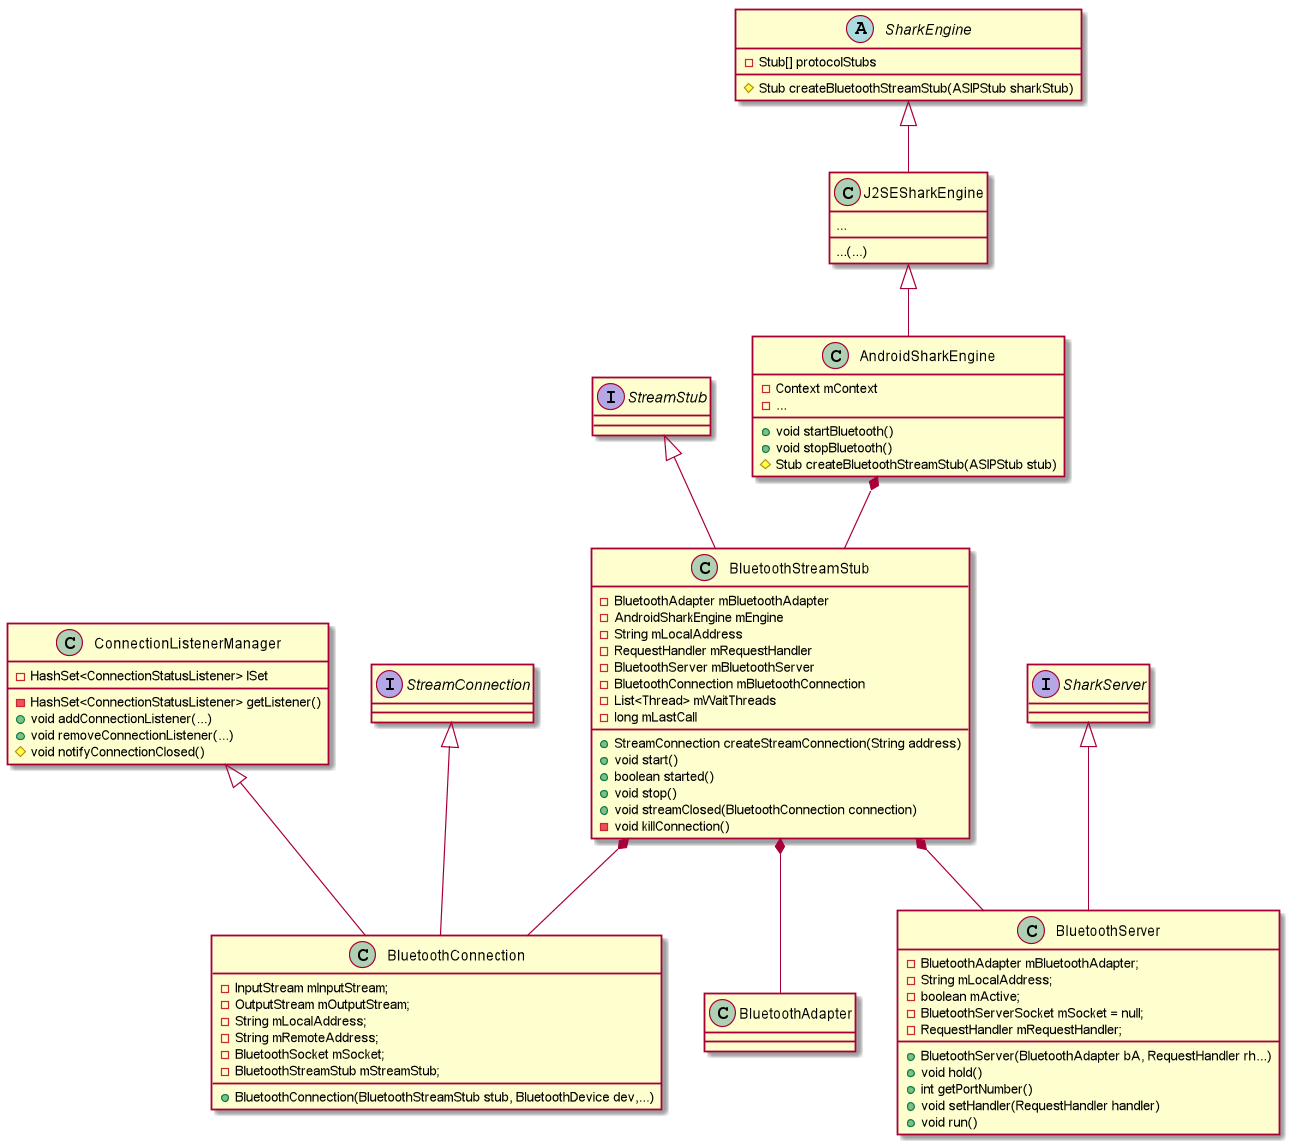
\includegraphics[width=1.1\linewidth]{bluetooth/images/bluetoothGesamt.png}}%
	\caption{Die Bluetooth Klassen im Überblick}
	\label{fig:bluetoothAll}
\end{figure}
Im Zentrum dieser Hierarchie steht die Klasse \textit{BluetoothStreamStub}. Eine Instanz dieser Klasse befindet sich als Attribut in der Klasse \textit{AndroidSharkEngine}, von der aus alle Protokolle wie NFC, Wifi-Direct oder Bluetooth gesteuert werden. Sie stellt daher auch Methoden wie \textit{startBluetooth()} oder \textit{stopBluetooth()} bereit. 





\subsection{Schnittstellendefinitionen}\label{ch:bluetoothinterfaces}
Anhand der Klassenhierarchie der Bluetooth-Komponente lässt sich erkennen, dass die folgenden drei Schnittstellen implementiert werden:
\begin{itemize}
	\item \textit{StreamStub}: Mit Hilfe von Implementierungen dieses Interfaces können streambasierte Ende-zu-Ende Verbindungen zwischen zwei Geräten hergestellt werden. Die Klasse BluetoothStreamStub öffnet und schließt daher die Verbindungen zu anderen Geräten per Bluetooth.
	\item \textit{StreamConnection}: Das Shark Framework definiert mit dem Interface StreamConnection das Verhalten einer streambasierten Verbindung zweier Geräte. Dieses Interface ist nicht zu verwechseln mit gleichnamigen Interface von Java ME. Klassen wie \textit{BluetoothConnection}, welche dieses Interface implementieren, bauen in ihren jeweiligen Konstruktur die Verbindung mit ihrem jeweiligen Protokoll auf. In der Klasse \textit{BluetoothConnection} erfolgt dies über das Bluetooth-Protokoll RFCOMM.
	\item \textit{SharkServer}: Eine dieses Interface implementierende Klassen wartet bei der bestehenden Verbindung auf Datenpakete, nimmt diese an und leitet sie an einen \textit{Request Handler} weiter. Die Klasse \textit{BluetoothServer} nimmt daher die Datenpakete an, die per bestehender Bluetoothverbindung eintreffen.

\end{itemize}


\section{Nutzung}
\subsection{Code}
Der Code dieser Komponente kann hier \url{https://github.com/SharedKnowledge/SharkNet-Api-Android/tree/master/api/src/main/java/net/sharksystem/api/shark/protocols/bluetooth} betrachtet werden. Wie auch die anderen Implementierungen von Übertragungsprotokollen, befindet sich auch die Bluetooth-Implementierung im Projekt \textit{SharkNet-Api-Android} im Package \textit{protocols}. 

\subsection{Deployment / Runtime}



\section{Test}



\section{Ausblick}
Es ist empfehlenswert, die von Android gestellten Bluetooth Klassen durch die dazu äquivalenten Bluetooth Low Energy (BLE) Klassen entweder zu ersetzen oder zumindest eine Alternative zu dem klassischen Bluetooth Package zu bieten. BLE verbraucht weniger Akkuleistung als das klassische Bluetooth, kann dafür aber nur eine geringere Menge an Daten pro Verbindung unterstützen. Da die mit SharkNet verschickten Nachrichten auch trotz der semantischen Annotationen nur wenige Kilobyte benötigen, stellt dies für SharkNet kein Hindernis dar.

